\documentclass{sig-alternate-ipsn13}

% \usepackage{amssymb,latexsym,amsmath,subfigure}     % Standard packages
% \usepackage{algorithm, algorithmic}
% \usepackage{color}
% \usepackage{xspace}
% \usepackage{enumitem}
\usepackage{booktabs}
\usepackage{epsfig,endnotes}
%\usepackage{usenix,epsfig,endnotes}
%\usepackage{amsmath,amssymb,alltt,times,mathptmx,graphicx}
\usepackage{amsmath,amssymb,times,graphicx,amsfonts}
\usepackage{courier,subfigure,color,sped,url,wrapfig}
\usepackage{xspace}
\usepackage{balance}
\usepackage{enumitem}
%\usepackage[square,comma,numbers,sort&compress]{natbib} %REMOVED. this package setting comflict with 'sig-alternate-10pt.cls'
%\usepackage[font=sf, labelfont={sf,bf}, margin=0.5cm]{caption}
%\usepackage[labelfont={bf},margin=0.3cm]{caption}
%\usepackage{citesort}

% \usepackage[colorlinks=true, linkcolor=blue,
%               citecolor=blue, urlcolor=blue,
%               ps2pdf,                %%% hyper-references for ps2pdf
%               bookmarks=true,        %%% generate bookmarks ...
% 	      bookmarksopen=true,
%               bookmarksnumbered=true,%%% ... with numbers
%   ]{hyperref}

% \hypersetup{ pdfcreator  = {LaTeX with hyperref package},
%                pdfproducer = {dvips + ps2pdf} }
               
%\let\url\nolinkurl % because dvips cannot break url across lines
%\hypersetup{
%pdfauthor   = {},
%pdftitle    = {},
%pdfsubject  = {},
%pdfkeywords = {},
%}

\urlstyle{rm}

\usepackage{lastpage}

%%It seems these two packages must be loaded AFTER hyperref
\usepackage{algorithm}
\usepackage[noend]{algorithmic}
%\usepackage{enumitem}

%%% Local Variables:
%%% mode: latex
%%% TeX-master: "paper"
%%% End:

%\usepackage[T1]{fontenc}
%\usepackage[utf8]{inputenc}
\usepackage{authblk}
% Useful macros for paper writing

\definecolor{brown}{cmyk}{0,0.81,1,0.60}
\definecolor{magenta}{rgb}{0.4,0.7,0}
\definecolor{gray}{rgb}{0.5,0.5,0.5}
\definecolor{red}{rgb}{1,0,0}
\definecolor{green}{rgb}{0.5,0,0.5}
\definecolor{blue}{rgb}{0,0,1}
\newcommand{\etc}{\emph{etc.}\xspace}
\newcommand{\ie}{\emph{i.e.,}\xspace}
\newcommand{\eg}{\emph{e.g.,}\xspace}
\newcommand{\etal}{\emph{et al.}\xspace}
\newcommand{\vlc}{vlc\xspace}
\newcommand{\SNOOZE}{Snooze\xspace}
\newcommand{\snz}{Snooze\xspace}
\newcommand{\POLICE}{Police\xspace}
\newcommand{\police}{Police\xspace}
\newcommand{\Police}{Police\xspace}
\newcommand{\PSTA}{Police Station\xspace}
\newcommand{\RTH}{\textbf{A}\xspace}
\newcommand{\ISI}{\textbf{B}\xspace}
%\newcommand{\reducefiguretopvmargin}{\vspace*{0ex}}
%\newcommand{\reducefigurebottomvmargin}{\vspace*{0.0ex}}
\newcommand{\reducefigurebottomvmarginsmall}{\vspace{-3mm}}
\newcommand{\reducefigurebottomvmargin}{\vspace{-4mm}}
\newcommand{\reducefigurecaptionmargin}{\vspace{-0mm}}
\newcommand{\reduceparavmargin}{\vspace*{0.0ex}}
%\newcommand{\reduceparavmargin}{\vspace*{-2.0ex}}
\newcommand{\reducesectionvmargin}{\vspace*{0.0ex}}
%\newcommand{\reducesectionvmargin}{\vspace*{-1.0ex}}
\newcommand{\reducevmarginsmall}{\vspace*{-.5ex}}
\newcommand{\reducevmarginone}{\vspace*{-1.0ex}}
\newcommand{\reducevmargintwo}{\vspace*{-2.0ex}}
\newcommand{\reducevmarginthree}{\vspace*{-3.0ex}}
\newcommand{\reducevmarginfour}{\vspace*{-4.0ex}}
\newcommand{\reducevmarginfive}{\vspace*{-5.0ex}}
\newcommand{\mypar}[1]{\vspace*{0.5ex}\noindent\textbf{#1}}
\newcommand{\mypari}[1]{\vspace*{0.5ex}\noindent\emph{#1}}

\newcommand{\spacesavecaption}[1]{\vspace*{0.0ex}\caption{#1}\vspace*{-3.5ex}}

\newcommand{\smallsection}[1]{\vspace*{1ex}\noindent\textbf{#1}}

% comment
\newcommand{\comment}[1]{{\color{gray}[\textsf{#1}]}}
\newcommand{\binliu}[1]{{\color{green}(KJ: #1)}}
\newcommand{\fei}[1]{{\color{red}(AS: #1)}}
\newcommand{\ramesh}[1]{{\color{blue}(RG: #1)}}
\newcommand{\yurong}[1]{{\color{brown}(SH: #1)}}
\newcommand{\camera}[1]{#1}

%\hyphenation{rate-allo-c-ation}

\newcommand{\equaref}[1]{Eq.~(\ref{eq:#1})}
\newcommand{\figref}[1]{\ref{fig:#1}}
\newcommand{\algref}[1]{Alg.~(\ref{alg:#1})}
\newcommand{\ruleref}[1]{\textsc{Rule}~\ref{rule:#1}}
\newtheorem{rul}{Rule}
\newcommand{\nonoverlapping}{\mbox{non-o}\-ver\-lap\-ping\xspace}
\newcommand{\interframe}{interframe\xspace}

\newcommand{\script}[1]{{{\cal{#1}}}}


\newtheorem{theorem}{Theorem}[section]
\newtheorem{lemma}[theorem]{Lemma}
\newtheorem{proposition}[theorem]{Proposition}
\newtheorem{corollary}[theorem]{Corollary}

% \newenvironment{definition}[1][Definition]{\begin{trivlist}
% \item[\hskip \labelsep {\bfseries #1}]}{\end{trivlist}}
% \newenvironment{example}[1][Example]{\begin{trivlist}
% \item[\hskip \labelsep {\bfseries #1}]}{\end{trivlist}}
% \newenvironment{remark}[1][Remark]{\begin{trivlist}
% \item[\hskip \labelsep {\bfseries #1}]}{\end{trivlist}}

\newcommand{\bm}[1]{\mbox{\boldmath{$#1$}}}
\newcommand{\ppcl}{Pickle\xspace}



%Figures

\newcommand{\scaleImage}[4]{
\begin{figure}[#1]
\centering
\includegraphics[width=#2\textwidth]{figs/#3}
\reducefigurecaptionmargin
\caption{#4\label{fig:#3}}
\reducefigurebottomvmarginsmall
\end{figure}
}

\newcommand{\scaleImageLabel}[5]{
\begin{figure}[#1]
\centering
\includegraphics[width=#2\textwidth]{figs/#3}
\reducefigurecaptionmargin
\caption{#4\label{fig:#5}}
\reducefigurebottomvmarginsmall
\end{figure}
}


\newcommand{\fullColumnFigs}[3]
{
\begin{figure*}[!tb]
  \centering
  {#1}
\reducefigurecaptionmargin
\caption{#2\label{fig:#3}}
\reducefigurebottomvmargin
\end{figure*}
}

\newcommand{\scaleTable}[4]{
\begin{table}[#1]
\centering
\includegraphics[width=#2\textwidth]{figs/#3}
\reducefigurecaptionmargin
\caption{#4\label{tbl:#3}}
\reducefigurebottomvmarginsmall
\end{table}
}

\newcommand{\oneColumnFigs}[3]
{
\begin{figure}[t]
  \centering
  {#1}
\reducefigurecaptionmargin
\caption{#2\label{fig:#3}}
\reducefigurebottomvmargin
\end{figure}
}

\newcommand{\subImage}[3]{% width, filename1, caption1, label1
    \hspace*{-2.0ex}
    \subfigure[#3]
    {
      \includegraphics[width=#1\textwidth]{figs/#2}
      \label{fig:#2}
    }
}

\newcommand{\subImagePadded}[5]{% figure_width, hpadding, filename1, caption1, label1
    \subfigure[#4]
    {
      \hspace{#2\textwidth}
      \includegraphics[width=#1\textwidth]{figs/#3}
      \hspace{#2\textwidth}
      \label{fig:#5}
    }
}

\newcommand{\subImageWithNoLable}[2]{% width, filename1, caption1, label1
      \includegraphics[width=#1\textwidth]{figs/#2}
}

%%% Local Variables: 
%%% mode: latex
%%% TeX-master: "paper"
%%% End: 


%%%%%%%%%%%
% Margins %
%%%%%%%%%%%
%\addtolength{\textwidth}{1.0in} \addtolength{\textheight}{1.00in}
%\addtolength{\evensidemargin}{-0.75in}
%\addtolength{\oddsidemargin}{-0.75in}
%\addtolength{\topmargin}{-.50in}


%%%%%%%%%%%%%%%%%%%%%%%%%%%%%%
% Theorem/Proof Environments %
%%%%%%%%%%%%%%%%%%%%%%%%%%%%%%
%\newtheorem{theorem}{Theorem}
%\newenvironment{proof}{\noindent{\bf Proof:}}{$\hfill \Box$ \vspace{10pt}}
\newcommand{\jyr}[1]{{\color{red}#1}}
\newcommand{\mscope}{MediaScope\xspace}
\newcommand{\crs}{Credit Reward Scheme\xspace}

%%%%%%%%%%%%
% Document %
%%%%%%%%%%%%
\begin{document}
\conferenceinfo{IPSN'13,} {April 8--11, 2013, Philadelphia, Pennsylvania, USA.}
\CopyrightYear{2013}
\crdata{978-1-4503-1959-1/13/04}
\clubpenalty=10000
\widowpenalty = 10000

\title{Demo Abstract: MediaScope: Selective On-Demand Media Retrieval from Mobile Devices\titlenote{\scriptsize Research was sponsored by the Army Research Laboratory and was
accomplished under Cooperative Agreement Number W911NF-09-2-0053.  The
views and conclusions contained in this document are those of the
authors and should not be interpreted as representing the official
policies, either expressed or implied, of the Army Research Laboratory
or the U.S. Government.  The U.S. Government is authorized to
reproduce and distribute reprints for Government purposes
notwithstanding any copyright notation here on.}}
\numberofauthors{6} %  in this sample file, there are a *total*
% of EIGHT authors. SIX appear on the 'first-page' (for formatting
% reasons) and the remaining two appear in the \additionalauthors section.
%
\author{
% You can go ahead and credit any number of authors here,
% e.g. one 'row of three' or two rows (consisting of one row of three
% and a second row of one, two or three).
%
% The command \alignauthor (no curly braces needed) should
% precede each author name, affiliation/snail-mail address and
% e-mail address. Additionally, tag each line of
% affiliation/address with \affaddr, and tag the
% e-mail address with \email.
%
% 1st. author
\alignauthor
Yurong Jiang\titlenote{\scriptsize The first two authors contributed equally to this work and their names are listed alphabetically by last name.}\\
       \affaddr{University of Southern California}\\
       \email{yurongji@usc.edu}
\alignauthor
Xing Xu \\
  \affaddr{University of Southern California} \\
  \email{xingx@usc.edu}
\alignauthor
Peter B. Terlecky \\
       \affaddr{City University of New York}\\
       \email{pterlecky@gc.cuny.edu}
\and
\alignauthor
Tarek Abdelzaher \\
       \affaddr{University of Illinois at Urbana-Champaign}\\
       \email{zaher@illinois.edu}
\alignauthor
Amotz Bar-Noy\\
       \affaddr{City University of New York}\\
       \email{amotz@sci.brooklyn.cuny.edu}
\alignauthor
Ramesh Govindan\\
       \affaddr{University of Southern California}\\
       \email{ramesh@usc.edu}
}

\maketitle
\begin{abstract}

Motivated by an availability gap for visual media, where images and
videos are uploaded from mobile devices well after they are generated,
we explore the \emph{selective,
  timely retrieval} of media content from a collection of mobile
devices.
%
We envision this capability being driven by \emph{similarity-based
  queries} posed to a cloud search front-end, which in turn
dynamically retrieves media objects from mobile devices that best
match the respective queries within a given time limit.
%
Building upon a crowd-sensing framework, we have designed and
implemented a system called \mscope that provides this capability.
%
\mscope is an extensible framework that supports nearest-neighbor and
other geometric queries on the feature space (e.g., clusters,
spanners), and contains novel retrieval algorithms that attempt to
maximize the retrieval of relevant information.
%
From experiments on a prototype, \mscope is shown to achieve
near-optimal query completeness and moderate overhead on mobile
devices..

\end{abstract}

\section {Introduction}
Cameras on mobile devices have given rise to significant
\emph{sharing} of media sensor data (photos and videos).
%
Users upload visual media to online social networks like
Facebook~\cite{facebook}, as well as to dedicated sharing sites like
Flickr~\cite{Flickr} and Instagram~\cite{instagram}.
%
However, these uploads are often not \emph{immediate}.
%
Camera sensors on mobile devices have been increasing in both image
and video resolution far faster than cellular network capacity.
%
More important, in response to growing demand and consequent
contention for wireless spectrum, cellular data providers have imposed
data usage limits, which dis-incentivize immediate photo uploading and
create an \emph{availability gap} (the time between when a photo or
image is taken and when it is uploaded).
%
To bridge this availability gap, and to enable this and other missed
opportunities, we consider a novel capability for selective and timely on-demand
retrieval of images from mobile devices.
%
Specifically, we develop a system called \mscope that permits
concurrent timely geometric queries in feature space on media data
that may be distributed across several mobile devices.
%
\mscope is an extensible framework that supports different kinds of
queries.
%
\mscope queries permit nearest-neighbor searches on image feature
spaces, \emph{spanners} that retrieve samples of images that span
the feature space, or \emph{cluster representatives} that are samples
of clusters in the feature space.
%
\mscope also addresses the timelines and computational complexity issues through the novel concurrent uploading scheme design and accuracy-complexity tradeoff.


\section{MediaScope Design}
MediaScope is a system that supports timely similarity-based queries
on media objects stored on mobile devices.
%
Mediascope is conceptually partitioned across a cloud component called
MSCloud, and another component called MS\-Mobile that runs on mobile devices.
%
This partitioned design leverages the computation and storage power of
clouds to support geometric queries on the feature space; mobile
devices provide sensing and storage for media objects.

These components interact as follows (Figure~\ref{fig:architecture}).
%
In the background, whenever participants take photos or videos, the
\emph{Feature Extractor} component of MSMobile continuously extracts
image and video features and uploads them to the \emph{MSCloudDB}.
%
Users (e.g., a security officer or a reporter) pose queries to MSCloud
using a standard web interface, possibly on a mobile device.
%
These queries are processed by the \emph{MSCloudQ} query processing
engine, which uses the features stored in the MSCloudDB to compute the
query results.
%
The results of the queries identify the media objects that need to be
retrieved from individual mobile devices.
%
In some cases, a media object may already have been retrieved as a
result of an earlier query; query results are also \emph{cached} in
MSCloudDB in order to optimize retrieval.
%
MSCloudQ coordinates with an \emph{Object Uploader} component on
MSMobile in order to retrieve query results.

MediaScope uses a publicly available crowd sensing platform called
Medusa~\cite{Medusa}, to enable programmed interaction between MSCloud and Medusa, and to support MediaScope's timeliness requirement, we made several modifications to Medusa Platform.
%
The most challanging component of MediaScope is support for concurrent queries, we designed a \emph{credit assigment mechanism}, the main idea is as follows, each query is awarded a certain amount of credit, and the query itself is responsible for assigned these amount of credit to the qualified objects given by the query optimizer, so each object of uploading request in MSMobile is associated with a credit, MSMobile is going to upload in a way that maximizing the total credit of uploadable objects.
%
Our current instantiation of MediaScope supports three qualitatively
different queries: nearest neighbor, clusters, and spanners. Detailed implementation is discussed in the full paper.

\begin{figure}
\centering
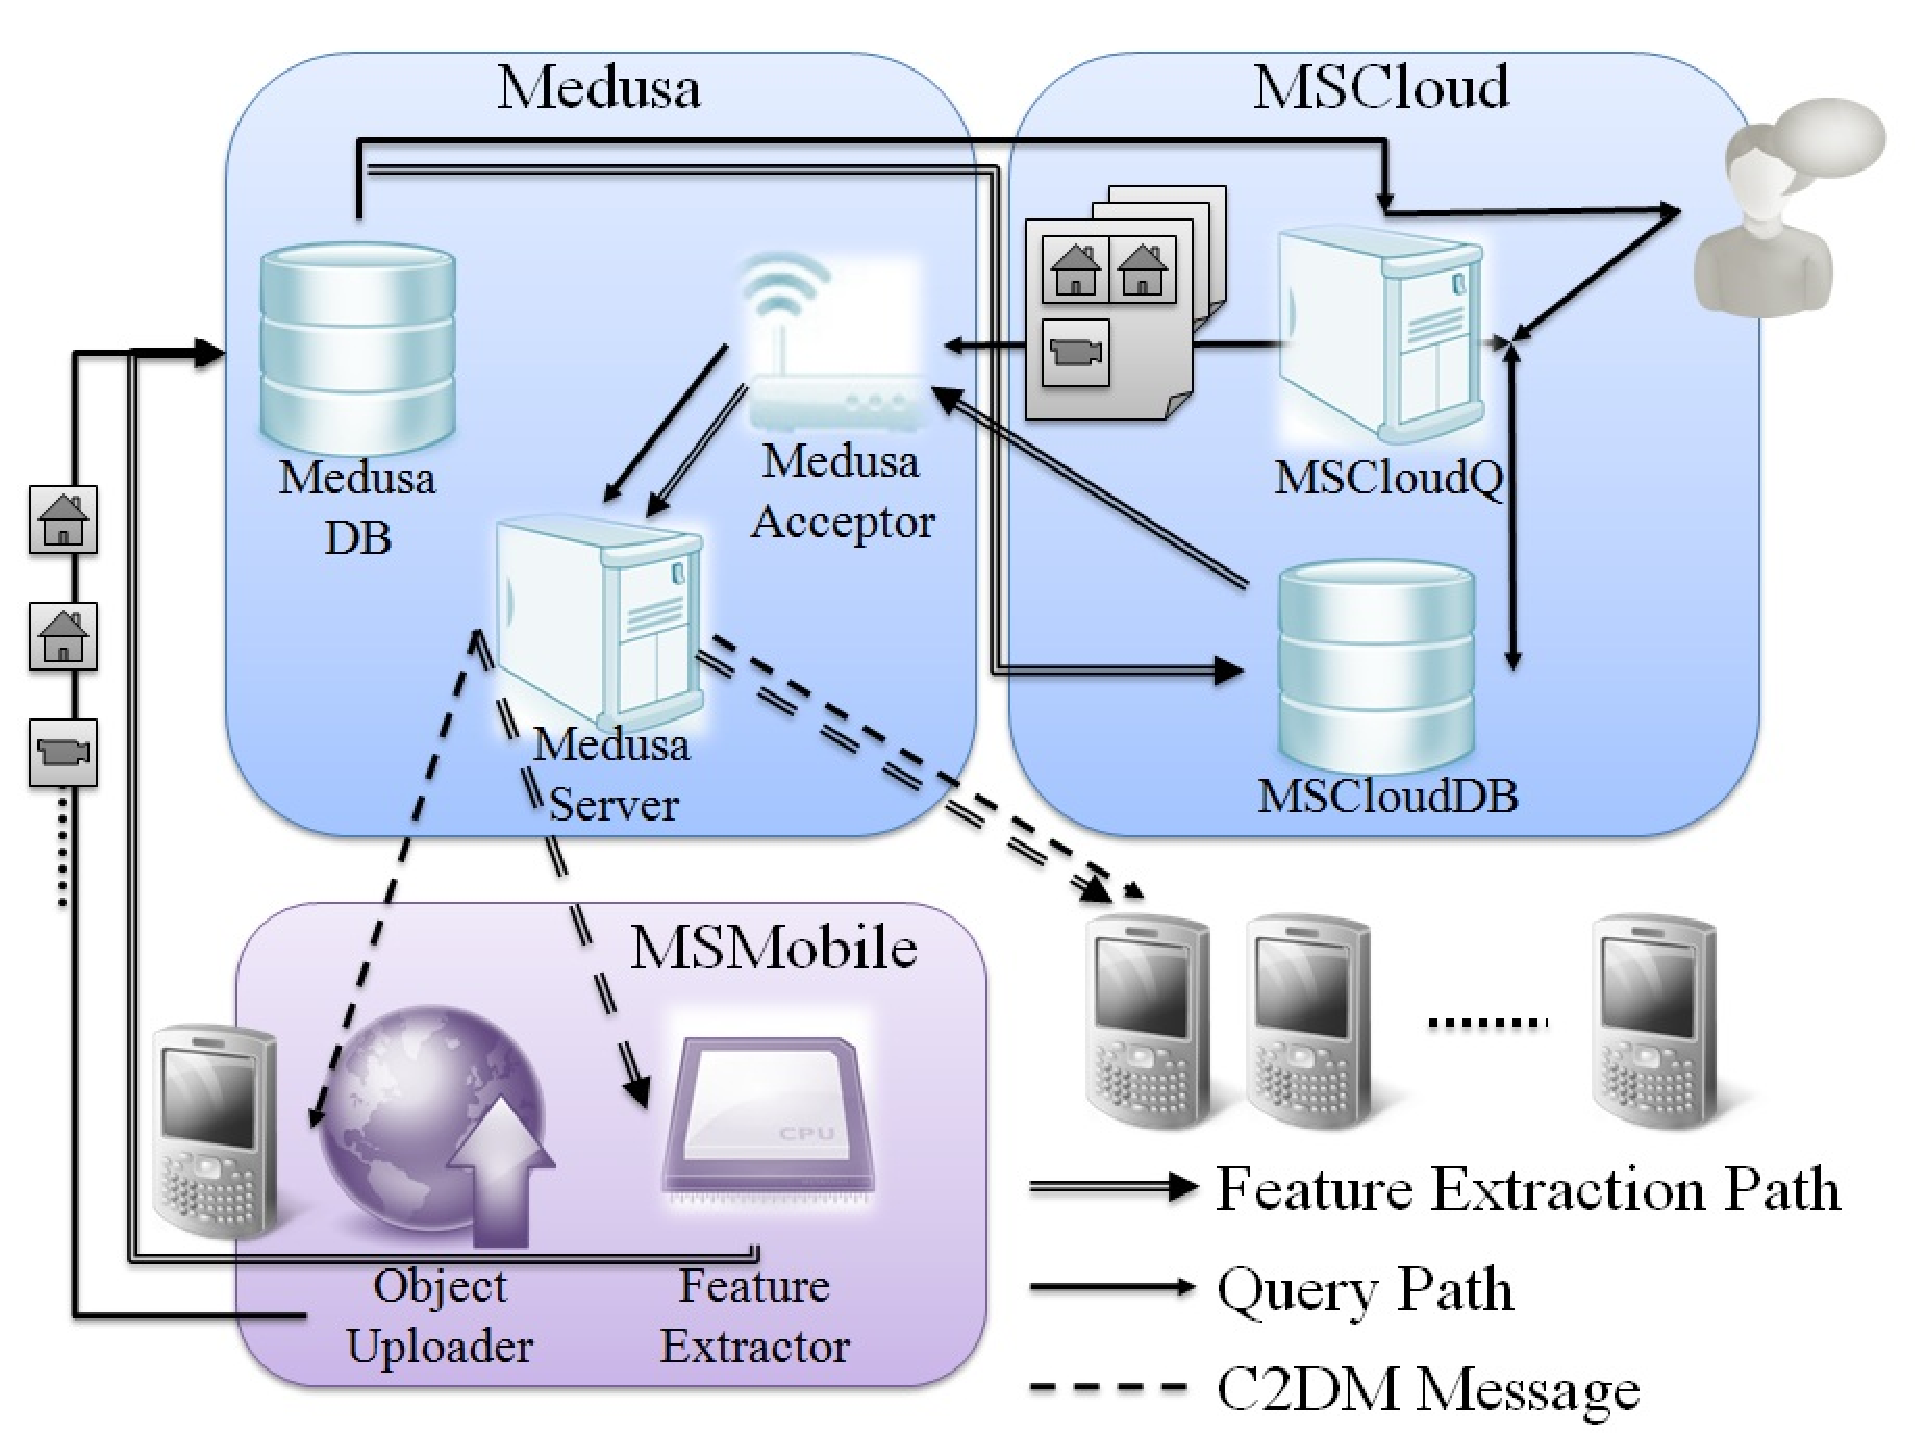
\epsfig{file=pics/architecture.eps, width=2.9in, height = 2in}
\caption{System Architecture Work Flow}
\label{fig:architecture}
\vspace{-0.5cm}
\end{figure}

\begin{figure}
\centering
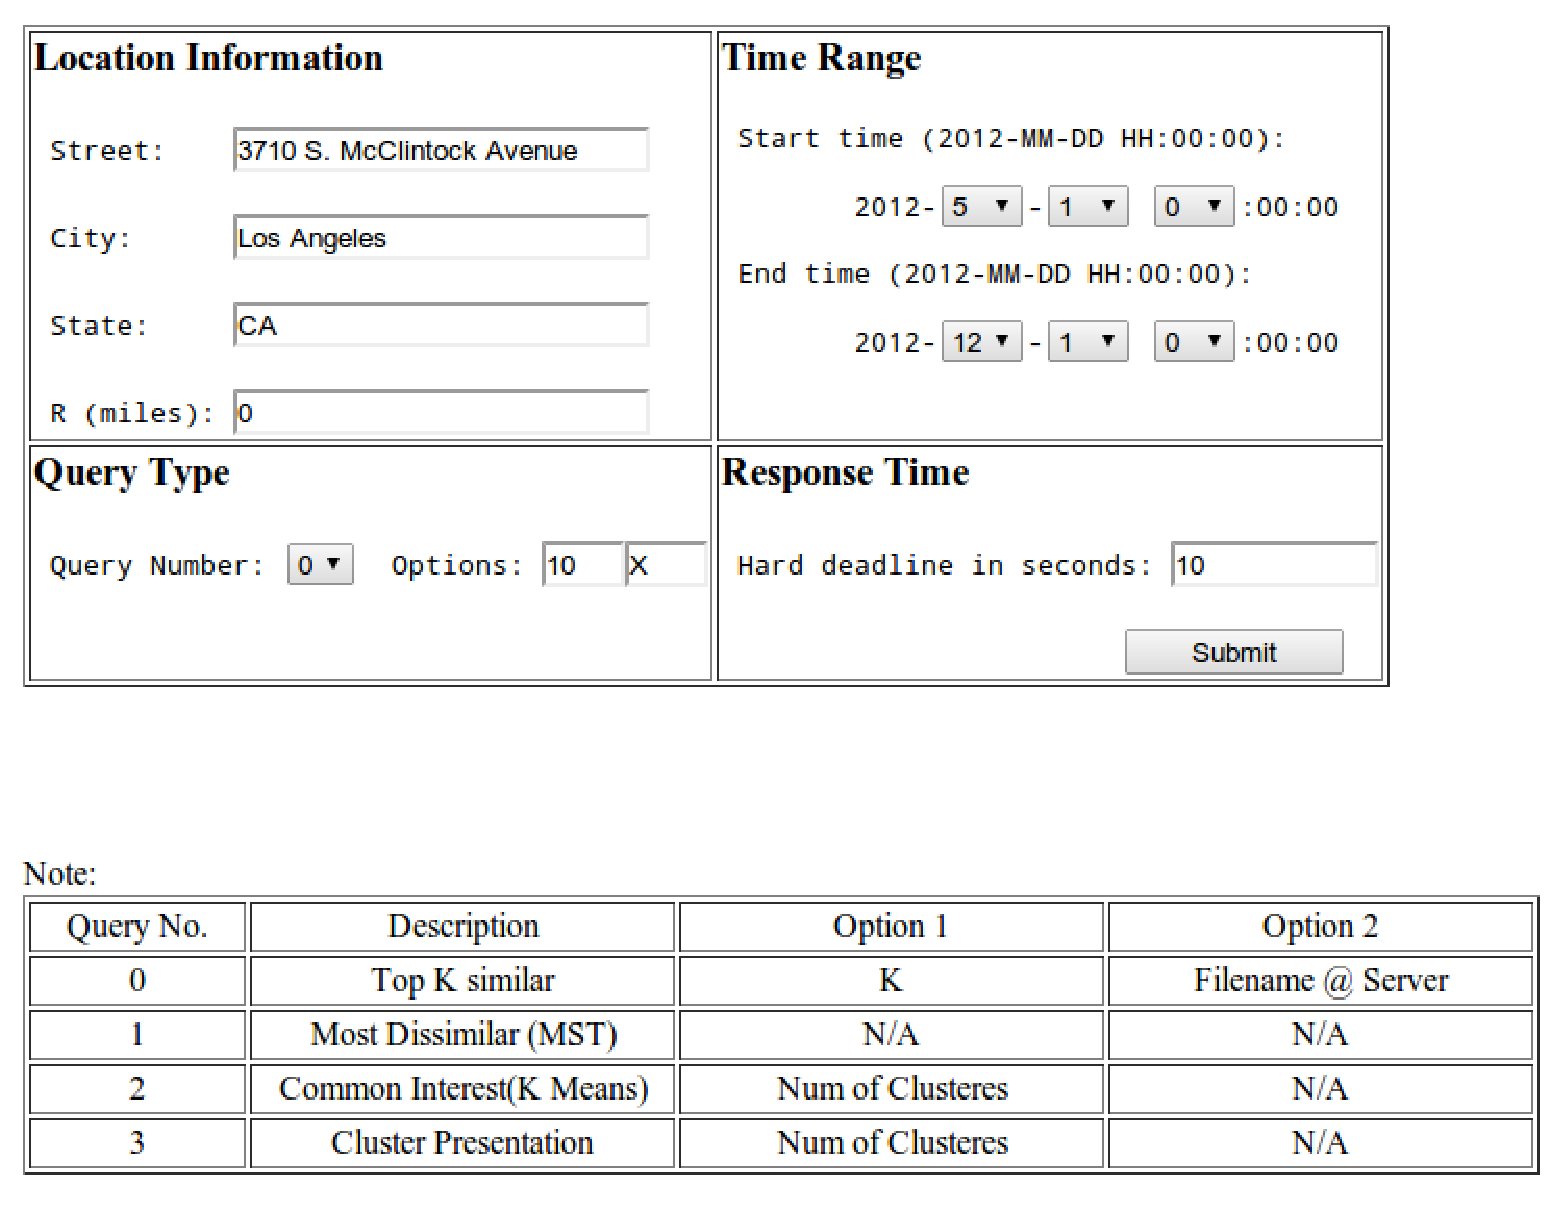
\epsfig{file=pics/queryinterface.eps, width=2.9in, height = 2in}
\caption{Query Interface}
\label{fig:interface}
\vspace{-0.8cm}
\end{figure}

\section{Demo Details}
We have built MediaScope prototype system using a commodity server machine and Android smartphones. The query interface of MSCloudQ is shown in Figure~\ref{fig:interface}. This demonstration will show the crucial steps of MediaScope: 1) the mobile device once capture an image, the corresponding feature will be extracted and uploaded to MSCloudDB automatically; 2) when MSCloud received query, it will select best media files and ask for uploading; 3) MSMobile will upload media files selected by MSCloud, and then MSCloud return results. For step 2), it is possible that MSCloud get concurrent queries (in the demo, we will issue multiple queries from different tabs of the browser); consequently, MSMobile will receive concurrent uploading tasks, sometimes this means that not all the uploading tasks can be completely uploaded before its timeliness bound and in this situation, the scheduling is critical for the sake of maximizing information (credit) collected.

\section{Related Work}
There are some other works focus on search over resources, \cite{sensorranking} deal with people-centric sensor data; however \mscope focuses on image search. \mscope is inspired by leveraging semantics of features \cite{crowdsearch,photonet}, techniques for content-based image retrieval from a centralized database of images \cite{faceted,virage,imgseek} and image retrieval from mobile devices \cite{content1,content2,content3}. Compared to existing works, \mscope uniquely supports searches on a cloud server, but where the content is stored on the mobile devices and is retrieved on demand. 

{
\balance\small{
\bibliographystyle{abbrv}
\bibliography{main}}}

\end{document}
